\chapter{Revisão Bibliográfica}
\label{revisao_bibliografica}

\section{Clusters}
\label{c2-clusters}

\textit{Clusters} são agregados de átomos ou moléculas, que variam desde dois a vários milhares de átomos e encontram-se na fronteira entre os átomos e o \textit{bulk}\footnote{\textit{Entende-se como "bulk" um conjunto de partículas grande o suficiente para que a média estatística de suas propriedades seja independente do número de partículas\cite{bulk}}}\cite{Heer,Brack}, por definição, eles se encontram em uma escala nanométrica ($ \leqslant 100$ nm).
No geral, os \textit{clusters} atômicos são classificados de acordo com seu tamanho: \textcolor{blue}{ muito pequenos, pequenos, médios ou grandes. Aglomerados classificados como muito pequenos e pequenos apresentam propriedades quânticas e possuem uma grande dependência com número de partículas que o compõe, essas propriedades não variam suavemente com seu tamanho, diferentemente dos \textit{clusters} médios e grandes.
Normalmente os \textit{clusters} são classificados pelo números de àtomos(n) que o compõem: muito pequenos ($3<n<12$), pequenos($13<n<100$), médios ($100<n<1000$) e grandes ($1000<n<10^8$).}
\textcolor{red}{Normalmente os \textit{clusters} são ditos pequenos quando contém da ordem de centas a mil partículas} Os nano-agregados considerados grandes possuem propriedades tendem a seguir as propriedades da matéria um \textit{bulk}.


Deixando de lado os casos limites que geram ambiguidades, a diferença entre \textit{cluster} e moléculas encontra-se no fato que estas, no geral, possuem composições específicas e bem definidas e, na grande maioria dos casos, suas estruturas também são bem definidas, tendo  assim um número restrito de átomos; diferente de um \textit{cluster} que, como exemplo, podemos citar um \textit{cluster} de prata que pode conter de 2, 15, 100, a qualquer número de átomos de prata, respeitando os limites impostos para que este ainda seja um \textit{cluster}. Esses, por sua vez, também não possuem uma estrutura única, como podemos ver na Figura \ref{fig:estrutura_cluster_ag}, e para sua maioria, à medida que o número de partículas do \textit{cluster} aumenta, o número de estruturas estáveis disponíveis torna-se mais abundante. 

\begin{figure}
  \centering
  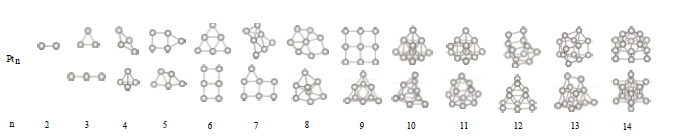
\includegraphics[width=1\textwidth]{images/clusters/estrutura_cluster_ag}
  \caption{ Exemplo de estruturas de \textit{clusters} de prata.\cite{dissertacao_anderson}  }
  \label{fig:estrutura_cluster_ag}
\end{figure}


 A análise das estruturas dos \textit{clusters} é fundamental para compreender suas propriedades e  dispor de seus potenciais tecnológicos, isso também torna-se muito importante para o domínio da estabilidade das nanopartículas. 


A análise da distribuição do tamanho dos \textit{clusters} pode prover critérios fundamentais para o entendimento das tendências estruturais e energéticas dos mesmos. Buscando entender melhor as transições das propriedades dos \textit{clusters}, segundo Bernd v. Issendorff (2009), podemos começar os estudos pensando em uma descrição simples, porém suficiente, do modo como se comportam os elétrons de um metal. Assumindo um sistema de elétrons livres, isto é, cujos elétrons da camada de valência se movem através de uma rede de metal infinita, agindo como partículas livres. Assim, as funções de onda eletrônicas são apenas ondas planas, tornando qualquer comprimento de onda possível.

Mudanças significativas ocorrem quando o metal possui dimensões nanoscópicas ou são nanopartículas. Agora, as funções de onda formam ondas estacionárias entre as superfícies da partícula, o que é possível somente para certos comprimentos de onda. Uma consequência direta é a discretização da densidade eletrônica de estados: a banda de valência contínua se divide em um número finito de estados. Este é o chamado efeito de tamanho, um efeito quântico que pode levar a mudanças significativas nas propriedades das partículas de metal. Pode-se esperar que tais efeitos possam ser mais claramente vistos para um metal que se aproxime do comportamento ideal dos elétrons livres \cite{capitulo_livro_shell}.

A Figura \ref{fig:transicao_cluster_solido} mostra a mudança das propriedades de um material enquanto \textit{clusters} e enquanto sólido massivo. \textcolor{blue}{Note que, as propriedades enquanto átomos ou moléculas que se comportam como \textit{clusters}, são não monotônicas, enquanto que apartir dos \textit{clusters} que se comportam como sólidos, as propriedades são monotônicas. Na região em que temos um regime de propriedades não monotônicas, propriedades incomuns para certos tipos de material podem surgir devido ao do confinamento quântico e dos efeitos de contorno. \textit{Clusters} de elementos não magnéticos tornam-se magnéticos, materiais semicondutores exibem propriedades metálicas, sistemas metálicos tornam-se semicondutores, a cor de partículas muda com tamanho, metais nobres tornam-se reativos e materiais frágeis tornam-se maleáveis.}\textcolor{red}{não dá para entender a relação do texto e a figura. Precisa falar da variação das propriedades monotônicas e não monotônicas}

\begin{figure}
  \centering
  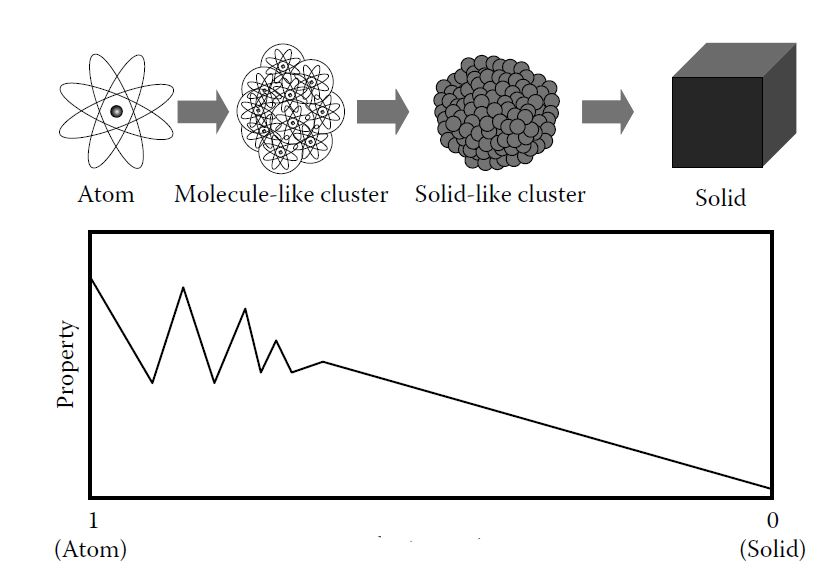
\includegraphics[width=0.7\textwidth]{images/clusters/atomo_cluste_solido}
  \caption{Esquema de transformação dimensional de átomos através de pequenos e grandes \textit{clusters} para o estado sólido. Quando os \textit{clusters} são pequenos cada átomo adicionado é importante, por isso as propriedades mudam
de forma abrupta com o tamanho. Quando os \textit{clusters} se tornam grandes,
propriedades mudam suavemente\cite{cap06_Nanophysics}. Adaptado.  }
  \label{fig:transicao_cluster_solido}
\end{figure}


Os estudos sobre as propriedades das nanopartículas indicam que a banda de condução eletrônica contínua de um sólido se divide em estados discretos se o metal for suficientemente pequeno. Para \textit{clusters} considerados grandes, a quantidade de níveis aumenta enquanto a largura do \textit{gap} diminui, levando à estrutura de banda do bulk.

Uma das mudanças de propriedade interessantes de serem estudadas é a função dielétrica do material. Quando os \textit{clusters} metálicos são considerados pequenos, a banda de condução se divide em níveis discretos separados por energias $\sigma$, que são maiores quando comparadas com as energias térmicas, sendo assim $\sigma>kT$, como pode-se ver na Figura \ref{fig:carac_metal}. Isso indica que as nanopartículas podem ter propriedades semelhantes a semicondutores, se aumentarmos um pouco seu tamanho, essas começaram a exibir comportamentos de pequenos pedaços do metal macroscópico.

\begin{figure}
  \centering
  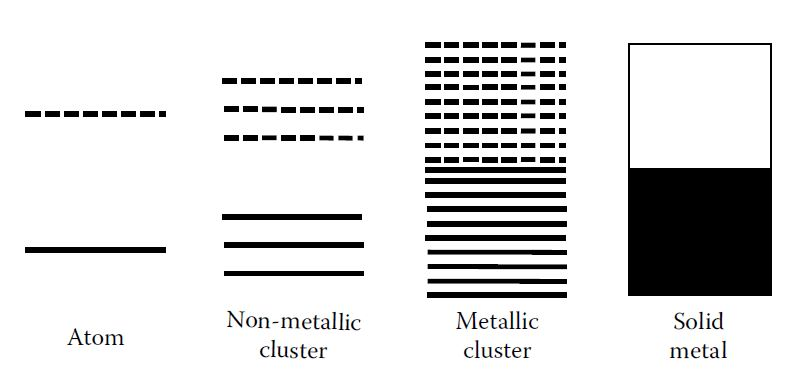
\includegraphics[width=0.65\textwidth]{images/clusters/carac_metal}
  \caption{ Esquema de transformação estrutural de energia desde de átomos de metal, pequenos e grandes \textit{clusters}, até o metal sólido. Abaixo de um certo tamanho de \textit{cluster}, no qual as bandas vazia e povoada se fundem, um \textit{cluster} de átomos de metal pode ter uma estrutura de energia semelhante a um semicondutor.\cite{dissertacao_anderson}  }
  \label{fig:carac_metal}
\end{figure}

Os \textit{clusters} podem ser produzidos a partir de diversos elementos da tabela periódica, como, por exemplo, metais alcalinos como sódio e potássio; metais alcalinos-terrosos, como cálcio, magnésio e bário; metais nobres, como ouro, prata  e cobre. Quando estudadas as nanopartículas de materiais que pertencem à mesma família, suas propriedades seguem o mesmo padrão.


\section{Espectro de massa das nanopartículas}
\label{sec:experimentos_teo}


Em 1984, Knight et al \cite{electronic_Shell_sodium} realizou um experimento com nanopartículas de sódio, com N átomos por conglomerado (N = 4-100), e foram encontrados padrões, com picos bem definidos, no espectro de massa de \textit{clusters} de Na em fase gasosa, podendo ser visto na Figura \ref{fig:espec_na}(a). Cada pico do espectro representa o número de 
aglomerados de um determinado N detectado. Note a presença de picos maiores, quando comparado com os outros picos, para certas massas correspondentes a N = $8, 20, 40, 58$ e $92$, onde podemos notar padrões. 




\begin{figure}
  \centering
  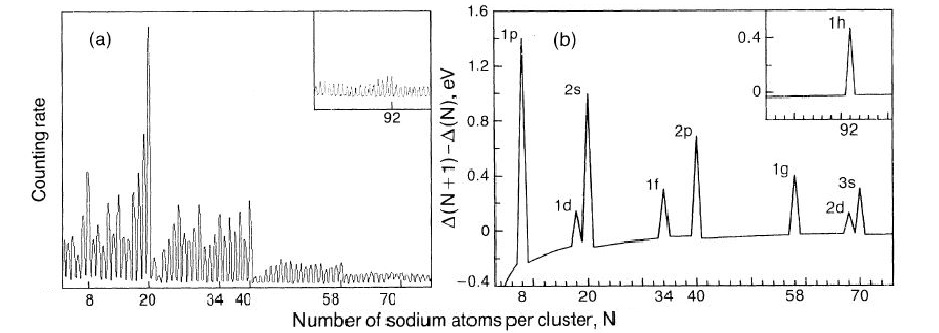
\includegraphics[width=1\textwidth]{images/clusters/NA_knight}
  \caption{(a) Espectro de massa de \textit{clusters} de sódio, N = 4-75.
  (b) A mudança calculada na diferença de energia eletrônica. Os picos protuberantes correspondem aos orbitais de casca fechada.\cite{electronic_Shell_sodium}  }
  \label{fig:espec_na}
\end{figure}


As características dos espectros de massa de outros metais alcalinos, e também dos metais nobres, seguem um padrão semelhante ao do sódio.

Em 1985, Katakuse et al \cite{KATAKUSE1985229} realizou um experimento com nanopartículas de cobre, prata e ouro, com $250$ átomos, e também foram encontrados padrões, com picos bem definidos em cada espectro de massa, como podemos ver nas Figuras \ref{fig:espec_ag},\ref{fig:espec_cu} e \ref{fig:espec_au}. No espectro de prata , podemos notar uma maior abundância nos picos como número de átomos iguais, $n= 3,9,21,35,41,59,93,139$ e $200$, já no espectro de cobre vemos que a abundância dos picos são nos \textit{clusters} com $n= 3,9,21,35,41,59,93,139$ e no espectro de ouro vemos que a abundância dos picos são nos \textit{clusters} com $n= 3,9,21,35,59,93,139$. \textcolor{blue}{Essa diferença ocorre devido as nanopartículas de prata, cobre e ouro serem ionizadas contendo um elétron a mais; como exemplos podemos citar o \textit{cluster} de prata 9:
\begin{equation*}
    Ag_{9} \to Ag_{8} + e^{-}
\end{equation*}} \textcolor{red}{Precisa explicar porque 3, 9, 21, ... ao invésde 2, 8, 20, ....}






\begin{figure}
  \centering
  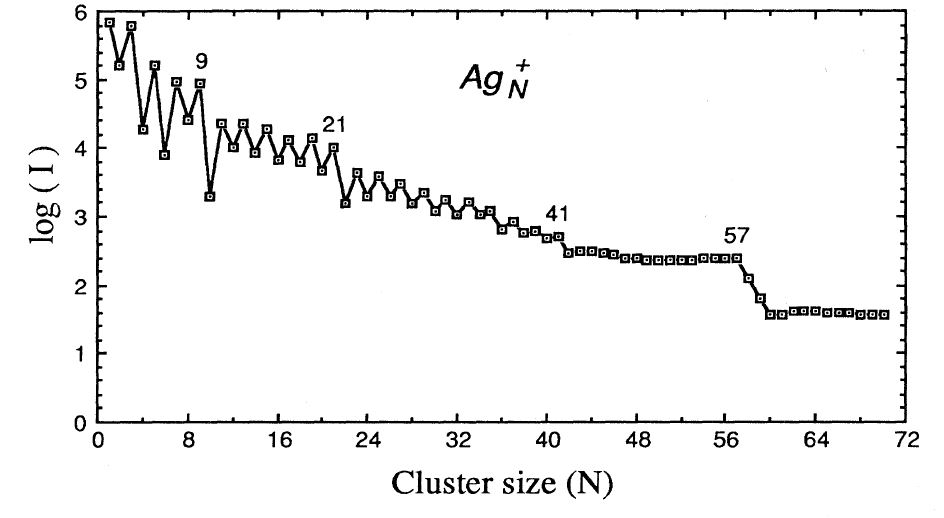
\includegraphics[width=0.7\textwidth]{images/clusters/espec_ag}
  \caption{(a) Espectro de massa de \textit{clusters} de prata \cite{Heer}.  }
  \label{fig:espec_ag}
\end{figure}

\begin{figure}
  \centering
  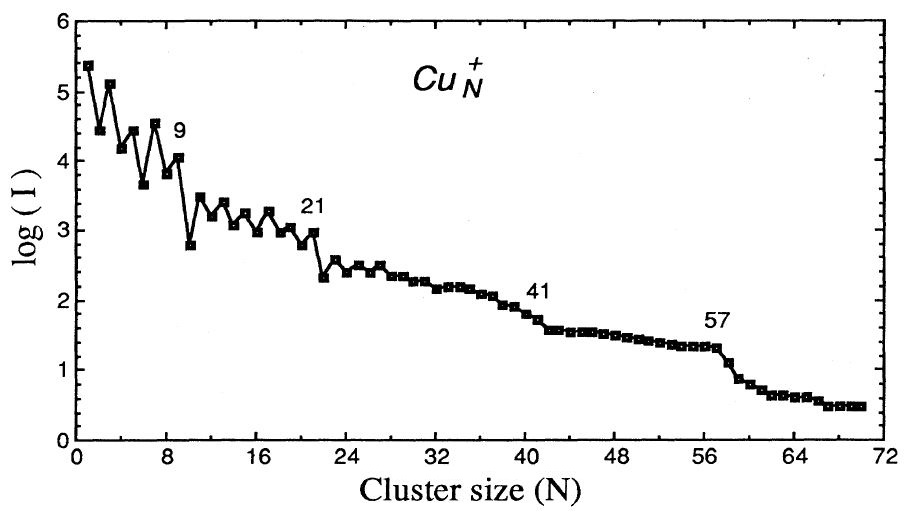
\includegraphics[width=0.7\textwidth]{images/clusters/espec_cu}
  \caption{(a) Espectro de massa de \textit{clusters} de cobre \cite{Heer}.  }
  \label{fig:espec_cu}
\end{figure}

\begin{figure}
  \centering
  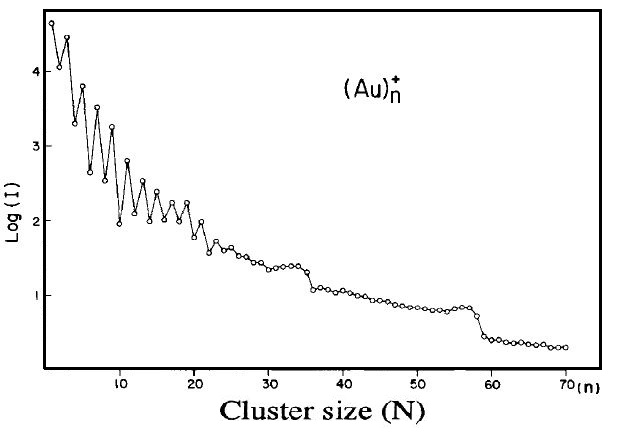
\includegraphics[width=0.65\textwidth]{images/clusters/espec_au}
  \caption{(a) Espectro de massa de \textit{clusters} de ouro \cite{KATAKUSE1985229}.  }
  \label{fig:espec_au}
\end{figure}




Os \textit{clusters} mais abundantes
nos espectros de massa foram apelidados de \textit{clusters mágicos}, ou \textit{clusters com números mágicos de átomos}, e são considerados relativamente mais estáveis. Podemos destacar a estrutura eletrônica dessas nanopartículas como a causa de maior estabilidade, como veremos a seguir.

Para explicar a ocorrência desses \textit{clusters mágicos}, foi suposto o efeito de preenchimento de camadas eletrônicas em que a combinação entre o espectro de estados
quantizados e o princípio de exclusão de Pauli resultam em efeitos de camada \cite{Brack}, ou seja, $1s^{2}$, $1s^{2}1p^{6}$, $1s^{2}1p^{6}1d^{10}$, $1s^{2}1p^{6}1d^{10} 2s^{2}$, … totalizando os números característicos do espectro de sódio mostrado na Figura \ref{fig:espec_na}. O modelo quântico de \textit{Jellium} \cite{Heer}, foi usado com sucesso para explicar a ocorrência desses \textit{clusters mágicos} \cite{capitulo_livro_shell}, como veremos na secção \ref{section_shell_model}.

Para as nanopartículas consideradas grandes, o padrão de números mágicos aparece diferente e, no geral, ele é atribuído como uma consequência do preenchimento de camadas geométricas ou poliédricas de casca, assim o \textit{cluster} assume geometrias que minimizam a relação átomo-superfície, uma vez que os átomos da superfície possuem um número menor de vizinhos do que os átomos internos, e o \textit{cluster} tende a preferir a estrutura de menor energia, maximizando a fração de átomo \textcolor{red}{em massa ?????}. Essa estrutura geométrica da \textcolor{red}{casca} é bem conhecida nos \textit{clusters} de gás, e é característica de interações de curto alcance nas quais a \textcolor{red}{tendência é o empacotamento do próximo do atomo juntamente - vamos conversar sobre essa parte} com a necessidade de minimizar a energia superficial \cite{capitulo_livro_shell}.


\section{Estrutura eletrônica \textit{shell model} para \textit{clusters} esféricos} \label{section_shell_model}

\textcolor{red}{melhorar esta frase} Pretendemos apresentar uma visão geral das características do sistema eletrônico \textit{shell model}.

O espectro de massa da \ref{fig:espec_na} sugere que os elétrons de valência nos \textit{clusters} de sódio são independentes e estão confinados em um potencial esfericamente simétrico. Assim como os átomos, com todas suas camadas eletrônicas preenchidas, as camadas eletrônicas de um \textit{cluster} com um número exato de elétrons para formar uma \textcolor{red}{estrutura geométrica poliédrica fechada} o torna muito estável. Quando um átomo for adicionado à nanoestrutura, seu elétron de valência ocupará um estado com energia maior e, assim, a estabilidade do \textit{cluster} será reduzida, reduzindo sua sua abundância no espectro, explicando a grande abundância após cada número de fechamento da camada. \cite{capitulo_livro_shell}.

Os números quânticos dos \textit{cluster} metálicos são caracterizados de modo que cada camada possui um número quântico radial \textit{n} e o momento angular \textit{l}. Para um dado número quântico \textit{l}, o estado mais baixo tem $n = 1$, e assim por diante \textcolor{red}{completar! ou retirar.}.


Uma primeira aproximação com abordagem quântica é o "Modelo de \textcolor{red}{melhor usar o jargão} Gota", que fornece uma descrição boa do comportamento observado na Figura \ref{fig:espec_na}. O \textit{cluster} é representado como uma esfera de raio \textit{R}, que está relacionada com número \textit{N} de átomos e o raio de Wigner-Seitz, $r_{s}$\cite{capitulo_livro_shell}\cite{livro_cap16_Misra2012527}.


\begin{equation}
\label{eq:raio_R}
    R = r_{s}(N)^{\frac{1}{3}}
\end{equation}

\textcolor{red}{O raio de Wigner-Seitz, $r_{s}$, é definido como o raio do volume ocupado por cada elétron de valência, que é equivalente ao volume ocupado por cada átomo em um metal monovalente.}
A estrutura interna do \textit{cluster} não é levada em consideração neste modelo, sendo ela equivalente à teoria de elétrons livres em sólidos. No entanto, a caixa sólida tem dimensões macroscópicas e níveis energéticos contínuos, enquanto o modelo para o \textit{cluster}, situado em nanoescala, os níveis de energia são discretos. Os primeiros níveis de energia para elétrons que não interagem em uma caixa esférica e o número de elétrons necessário para o preenchimento completo das camadas é $n= 2,8,18,20,34,40,58$ \cite{livro_cap16_Misra2012527}. Note que esses números condizem com os picos de maior abundância apontados no espectro da Figura \ref{fig:espec_na}.






Para o modelo de concha esféricas, os núcleos iônicos são substituídos por carga positiva uniforme de raio \textit{R}, os elétrons são tratados como partículas livres, movendo-se em um potencial parametrizado. O parâmetro básico do modelo é o raio de Wigner-Seitz, e a função onda para um potencial esfericamente simétrico pode ser escrita como:

\begin{equation}
    \psi_{ n,l,m}(r, \theta, \phi) = R_{nl}(r)Y_{lm}(\theta, \phi)
\end{equation}

Existem três potenciais úteis para o estudo da física de \textit{cluster}: potencial do oscilador harmônico, potencial esférico de poço quadrado e potencial Woods-Saxon. Estes potenciais são mostrados graficamente na Figura \ref{fig:pocos}. \textcolor{red}{A figura ficou muito longe.}

\subsubsection{Potencial do Oscilador Harmônico:}

O potencial mais simples é o potencial do oscilador harmônico $V_{r}$:

\begin{equation}
    V(r)= \frac{1}{2}m\omega_0r^2
\end{equation}

\noindent
o potencial do poço \textcolor{red}{quadrado esférico (constante para $r<R$ e infinito para os demais)}. Como podemos ver na primeira coluna da Figura \ref{fig:pocos}, os níveis de energia para o potencial do oscilador harmônico são igualmente espaçados, altamente degenerados  \textcolor{red}{e são rotulados pelo número quântico \textit{v}}.


A energia do potencial do oscilador harmônico é dada por:

\begin{equation}
    E_{v}= \left(\frac{3}{2}+v\right)h\omega_0
\end{equation}

Os números quânticos $(n,l)$ podem ser usados para qualquer potencial esfericamente simétrico. Assim, todos os orbitais com o mesmo valor de $(2n+l)$ são degenerados e as energias são escritas em termos do único número quântico $(2v+l-2)$ \textcolor{red}{que é?}. A energia potencial devido à carga de fundo é \cite{livro_cap16_Misra2012527}:
\begin{equation}
    \hbox{V}(r)
= \left\{ \begin{array}{lll}
\frac{3e^2N}{8\pi\epsilon_0R^3}\left(\frac{r^2}{3}-R^2\right) & \hbox{se} & r<R \\
e^2 Z & \hbox{} &  \\
\frac{e^2N}{4\pi\epsilon_0r} & \hbox{se} & r > R
\end{array}\right.
\end{equation}

\subsubsection{\textcolor{red}{Potencial Esférico de Poço Quadrado:}}

O potencial esférico de poços quadrados é descrito por:



\begin{equation}
 V(r) = \left\{\begin{array}{lll}
C & \hbox{se} & r < R \\
\infty & \hbox{se}  & \forall r
\end{array}\right.
\end{equation}



\noindent
em que C é uma constante. A função de onda radial $R_{nl}(r)$ para o potencial do poço quadrado é escrita em termos da função de Bessel esférica $j_{l}(K_{nl}R)$, em que

\begin{equation}
    K_{nl}=\left[\frac{2m|E|}{\hbar^2}\right]^{\frac{1}{2}}
\end{equation}

Os níveis de energia são determinados pelas condições de contorno $j_{l}(K_{nl}R)=0$ e, para cada $l$, o primeiro zero de $j_l$ é dado o número quântico $n = 1$, o segundo $n = 2$, e assim por diante. A ordem dos níveis de energia (que são emprestados da física nuclear e são diferentes da física atômica) são $1s$, $1p$, $1d$, $2s$, $1f$, $2p$, $1g$, $2d$,... Se duas soluções tiverem o mesmo número de nós radiais, aquela com maior $l$ terá maior energia. Nessa notação, o número quântico principal em física atômica é igual a $n + l$. O interior do \textit{cluster} será eletricamente neutro se incluirmos a contribuição da correlação de troca para o potencial eletrostático dos elétrons, e o potencial efetivo será quase constante. \textcolor{red}{O potencial do poço quadrado representa essencialmente esse fenômeno} \cite{livro_cap16_Misra2012527}.


\subsubsection{Potencial de Woods–Saxon:}

Em seu artigo, Knight et al\cite{electronic_Shell_sodium} utiliza o potencial de Woods-Saxon para realizar a análise dos espectros de massa de sódio mostrados na Figura \ref{fig:espec_na}\cite{livro_cap16_Misra2012527}, uma vez que ele é o potencial que melhor produz uma representação fenomenológica um potencial plano no centro de \textit{cluster} arredondado nas bordas. Este potencial é descrito por:

\begin{equation}
    U(r)=\frac{-U_0}{exp[(r-R)/\epsilon]+1}
\end{equation}


$U_0$ é a soma da energia de Fermi e a função de trabalho do metal a \textcolor{red}{granel}. $R$ é determinado pela equação \ref{eq:raio_R}. O parâmetro $\epsilon$ é usado para corresponder à variação do potencial na superfície. Para este potencial, não existem soluções analíticas.


Uma comparação entre os três potenciais apresentados pode ser vista na Figura \ref{fig:pocos}. Nela podemos ver que a degenerescência dos estados do potencial Woods-Saxon é semelhante a do potencial do poço quadrado, mas a ordenação dos níveis de energia são diferentes.

 Note também que os níveis com o mesmo momento angular são interligados. Pode-se ver que a sequência de níveis depende do potencial radial. Isso influi nos números “mágicos”, ou seja, nos números de elétrons para os quais os \textit{clusters} são especialmente estáveis. Nos níveis, os números de elétrons são: 2 elétrons preenchem o nível $1s$, 8 elétrons preenchem as camadas $1s$ e $1p$ e assim por diante.
 
 Os \textit{clusters} mais estáveis são aqueles com um nível completamente preenchido (chamado de casca fechada) e um grande espaço entre o nível ocupado mais alto e o nível mais baixo não ocupado. Portanto, os números de elétrons $34$ e $58$ são números “mágicos” do potencial quadrado, mas não do potencial Woods–Saxon. Os números $20$ e $40$ são fortemente “mágicos” para o oscilador harmônico e o potencial Woods–Saxon, mas menos para o potencial da caixa. Então, quais tamanhos de \textit{clusters} são especialmente estáveis depende fortemente do potencial radial, que pode ser diferente para diferentes metais.
 
Os números observados para 
\textit{clusters} de sódio na Figura \ref{fig:espec_na} $(8, 20, 40, 58)$ indicam que o potencial efetivo de partícula única está entre uma caixa e um potencial Woods–Saxon. Mas o mais importante é o acordo desses números com as previsões do modelo simples, o modelo de elétrons livres é capaz de descrever sistema eletrônico de \textit{clusters} de sódio \cite{livro_Clusters_Fullerenes}.

\begin{figure}
  \centering
  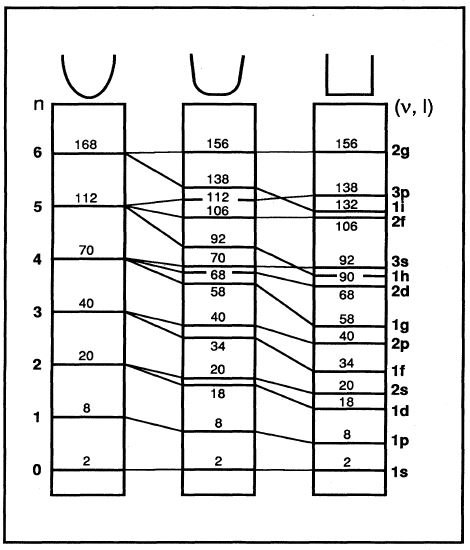
\includegraphics[width=0.5\textwidth]{images/clusters/pocos}
  \caption{Comparação dos potenciais (a) harmônico, (b) Woods-Saxon e (c) poço quadrado. \cite{Heer}}
  \label{fig:pocos}
\end{figure}

Em contrapartida, os "números mágicos"\ para os espectros de prata, cobre e ouro, mostrados nas Figuras \ref{fig:espec_ag},\ref{fig:espec_cu} e \ref{fig:espec_au}, ocorrem em
$9, 21, 35,...$ , diferente dos \textit{clusters} de sódio. Eles possuem as camadas 3d, 4d e 5d, com a camada d preenchido com 10 elétrons e um único elétron de valência. No experimento de Katakuse et. al. 1985,  os \textit{clusters} foram produzidos carregados positivamente e, assim, o número de elétrons em um aglomerado era $N - 1$, desta forma os números mágicos correspondentes às cargas eletrônicas de conchas estão coerentes com os resultados experimentais \cite{Heer}.

Comparando os espectros de sódio com os espectros dos metais nobres apresentados, vemos que neles a estrutura fina é dominada por um alternância par-ímpar nas intensidades, enquanto o espectro de sódio reflete a estrutura da subcamada prevista neste modelo. 




